\documentclass[10pt,a4paper]{article}

\usepackage[utf8]{inputenc}
\usepackage{hyperref}


\usepackage{tikz}
\usepackage{tikz-uml}
\usepackage[american voltages,siunitx]{circuitikz}
\usepackage{siunitx}

\usepackage{pgfplots}

\sisetup{binary-units, per-mode=symbol}

\usepackage[nomessages]{fp}

\usetikzlibrary{shapes,arrows,positioning}
% Define block styles
\tikzstyle{decision} = [diamond, draw, fill=blue!20, 
text width=4.5em, text badly centered, node distance=3cm, inner sep=0pt]

\tikzstyle{block} = [rectangle, draw, 
text width=2cm, text centered, rounded corners, minimum height=2em, node distance=1.5cm]

\tikzstyle{line} = [draw, -latex']

\tikzstyle{cloud} = [draw, dashed, ellipse, node distance=3cm,
minimum height=2em]

%\pagenumbering{Roman}
\pagenumbering{arabic}

\tikzstyle{icdev}=[draw, text width=6em, minimum height=8em]

% -------

\begin{document}



\newpage
\tableofcontents
\newpage


\section{Introduction}
This projects tries to use an Arduino\footnote{\url{http://www.arduino.cc}} Uno to transfer the screen output of a Raspberry Pi to one or more addressable LED stripes. The Raspberry Pi screen is read out using boblight\footnote{\url{code.google.com/p/boblight/}} and transfers a color array via UART to the Aruino, which creates the output for the LED stripe(s). In this project, the WS2811\footnote{\url{www.adafruit.com/datasheets/WS2811.pdf}} LED-controller is used.

\begin{figure}[htb]
\center
	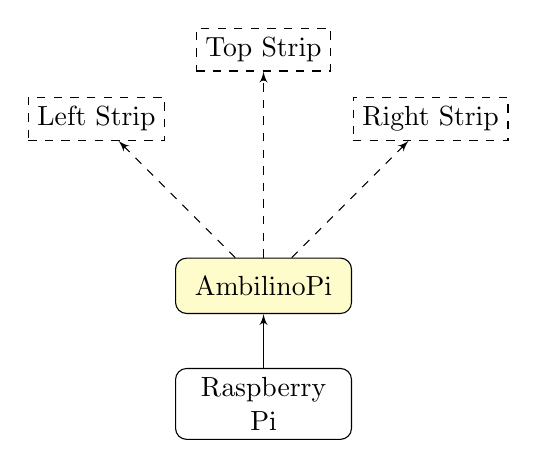
\begin{tikzpicture}[node distance = 3cm, auto]
	\node[block] (raspi) {Raspberry Pi};    
	\node[block, above of=raspi, fill=yellow!20] (AmbilinoPi) {AmbilinoPi};  		
	\node[rectangle, draw, dashed, above of=AmbilinoPi] (TStrip) {Top Strip};  			
	\node[rectangle, draw, dashed, above left of=AmbilinoPi] (LStrip) {Left Strip};  			
	\node[rectangle, draw, dashed, above right of=AmbilinoPi] (RStrip) {Right Strip};  				
%	\node[block, below of=TLed Strip, yshift = 7em, minimum height=4em] (TV) {TV};  				
% PATHS		
	\path [line, dashed] (AmbilinoPi) -- (LStrip);		
	\path [line, dashed] (AmbilinoPi) -- (TStrip);		
	\path [line, dashed] (AmbilinoPi) -- (RStrip);				
	\path [line] (raspi) -- (AmbilinoPi);	
		  
	\end{tikzpicture}
	\label{fig:overview}
	\caption{General Program Flow}
\end{figure}

\subsection{Eclipse Arduino IDE}
I used the Eclipse Arduino IDE \footnote{\url{www.baeyens.it/eclipse/}} for creating the Arduino Software. 

\begin{figure}[!ht]
\center
	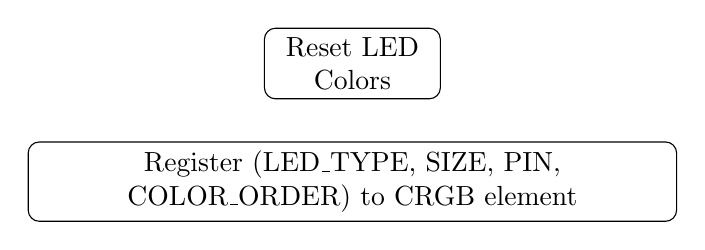
\begin{tikzpicture}[node distance = 3cm, auto]
	\node[block] (reset) {Reset LED Colors};    
	\node[block, text width = 8cm, below of=reset] (reset) {Register (LED\_TYPE, SIZE, PIN, COLOR\_ORDER) to CRGB element};    	

	
	
% PATHS		
	%\path [line] (setup) -- (values);		

		  
	\end{tikzpicture}
\end{figure}

\section{Setup}
\subsection{Hardware}

\subsubsection{Power consumption}

The power consumption of an all white LED strip can be calculated using the equation

\begin{equation}
	I_{LED Strip} = 3 * \SI{0.02}{\ampere} * n_{LED}
\end{equation}
So for 60 LEDs you would get a power consumption of \SI{3.6}{\ampere}! Inappropriate power sources result in LED flickering or other unexpected effects. 

\subsubsection{Board Schematic}

The basic schematic of the circuit looks like this:

\begin{figure}[!htb]
		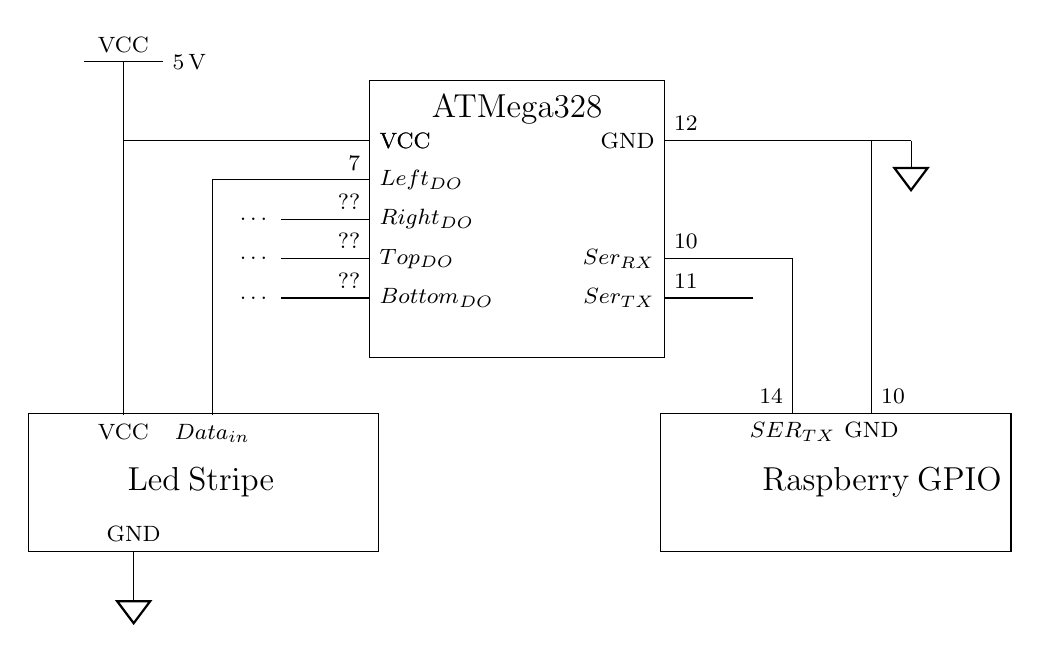
\begin{tikzpicture}[every node/.style = {font = \footnotesize}, transform shape]
	
	    \node (ATMega328) [icdev, text width=10em, minimum height=10em] {};
	    \node (title) [above of=ATMega328, yshift=0.4cm] {\large ATMega328};
	    
	    \node (raspi) [icdev, text width=12em, minimum height=5em, below right of=ATMega328, yshift = -7.5em, xshift = 9.5em, align=center] {\hfill \large Raspberry GPIO};
	
	    
	    \node (left) [icdev, text width=12em, minimum height=5em, left of=raspi, xshift = -20em] {\hspace{3.5em} \large Led Stripe};    
	    
	    %atmega
	    \draw (-5,1) -- (-1.87,1) node[right]{VCC} node[above left]{}
			  (-3.87,-2.48) node[below]{$Data_{in}$} |- (-1.87,0.5) node[right]{$Left_{DO}$} node[above left]{7}
			  (-3,0) node[left]{\dots} -- (-1.87,0) node[right]{$Right_{DO}$} node[above left]{??}
			  (-3,-0.5) node[left]{\dots} -- (-1.87,-0.5) node[right]{$Top_{DO}$} node[above left]{??}
			  (-3,-1)  node[left]{\dots} -- (-1.87,-1) node[right]{$Bottom_{DO}$} node[above left]{??};
	
	    \draw (5,1) -- (1.87,1) node(atgnd)[left]{GND} node[above right]{12}
			  (3.5,-2.46) node[below]{$SER_{TX}$} node[above left]{14} |- (1.87,-0.5) node[left]{$Ser_{RX}$} node[above right]{10}
			  (3,-1) node[sground, right of=atgnd, xshift=2.6cm] {} -- (1.87,-1) node[left]{$Ser_{TX}$} node[above right]{11};
		
		%rpi
		 \draw (4.5,1) -- (4.5,-2.46) node[below]{GND} node[above right]{10};
		
		%stripe
		 \draw (-4.87,-4.22) node[above]{GND} -- (-4.87,-4.5) node[sground] {}
			   (-3,1) -- (-1.87,1) node[right]{VCC} node[above left]{};
			  % (-4.87,-2.48) node[below]{AAA} |- (-4.87,0.5) node[vcc]{BBB} node[above left]{12};	
	
	  \draw  (-5.5,2) --  node[anchor=south] {VCC} (-4.5,2)  node[anchor=west] {\SI{5}{V}};
	  \draw (-5,2) to (-5,-2.48) node[below]{VCC};
	
	 
	\end{tikzpicture}
	\label{fig:schematic}
	\caption{Schematic of Arduino, Led Stripes and Raspberry GPIO}
\end{figure}	
%


	%\includegraphics[scale=0.5]{rpi-gpio.png}

\subsection{Boblight}

The Boblight software is used on the Raspberry inside the XBMC distribution like Openelec\footnote{\href{http://www.openelec.tv/}{http://www.openelec.tv/}}. The LED setup has to be configured inside the configuration file which is loaded at startup of boblightd. You can use a configuration generator which can be downloaded at \href{http://www.sedu-board.de/sedu-ambilight/howto-boblightconfigtool/}{sedu-board.de}. Refer to the boblight documentation\footnote for details. In general, the file should look like this: 

\begin{verbatim}
[device]
name ambilight
# Where to put signal -> UART
output /dev/ttyAMA0
# channels = number of leds * 3
channels 54
# use type momo
type momo
# interval sets the updaterate in microseconds
interval 10000000
# prefix = "SYNC"
prefix 53 59 4E 43
# postfix = "\r\n"
postfix 0D 0A
# 38400 -> 30ms per frame min
# UART BAUDrate
rate 38400

[color]
name red
rgb FF0000
adjust          0.5
blacklevel      0.1
gamma           2.3

[color]
name green
rgb 00FF00

[color]
name blue
rgb 0000FF

[light]
name led0000
color red ambilightleft 1
color green ambilightleft 2
color blue ambilightleft 3
hscan 0 10
vscan 0 6
\end{verbatim}
\label{fig:boblightconfexample}
After the general setup, you can tweak the colors of your stripe with adjust, blacklevel and gamma. When you are finished, you can set the individual LEDs and their corresponding screen rectangles.

\subsection{Arduino}

The main purpose of the Arduino firmware is the translation of the UART output of the Raspberry to the desired LED strips. Another thing is the smoothing of incoming colors so that the LEDs do not look too 'agressive'. 

% DEFINES for calculation
\def \CaptureBaudrate {38400}
\def \nLED {60}

\subsubsection{Capture Rate}
The time between two successive frames has an lower limit due to maximum serial readout. Currently it is used \verb|8-N-1|\footnote{\url{http://www.modemhelp.net/faqs/8n1.shtml}}. So there are \SI{10}{\bit} needed to transmit \SI{8}{\bit} of usable data. This means, that only $P_{8N1} = \SI{80}{\percent}$ of the transmission rate can be used. The minimum LED update frame time regarding the number of used LEDs and a specific Baudrate can be calculated:
	\begin{equation} 
T_{cap}(R_{Baud}, n_{LED}) = \frac{\SI{24}{\bit} * n_{LED}}{R_{Baud} * P_{8N1}} 
	\end{equation}
The \SI{24}{\bit} represent the size of a single color sent to one specific LED. Setting $n_{LED} = \nLED$ and $R_{Baud}$ = \SI{\CaptureBaudrate}{\bit\per\second}, $T_{cap}$ results in 

	\FPeval{\Tmin}{round(1000 * 24 * \nLED / (0.8 * \CaptureBaudrate),2)}
	\FPeval{\Reff}{clip(0.8 * \CaptureBaudrate)}	

	\begin{equation} 
T_{cap}(\SI{\CaptureBaudrate}{\bit\per\second}, \nLED) = \SI{\Tmin}{\ms}
	\end{equation}
This results in a maximum theoretical frame rate of 	
	
	\FPeval{\Tmin}{round(1000 / \Tmin,2)}	
	
	\begin{equation} 
R_{cap} = {T_{cap}}^{-1} = \SI{\Tmin}{\Hz}
	\end{equation}	
It is recommended to guarantee $R_{cap} \geq \SI{15}{\Hz}$ for sufficiently dynamic screen capturing.

\subsubsection{LED Smoothing}
	
	Putting the input colors directly on the LEDs can look quite aggressive and non-natural. It is recommend to use some kind of low pass filter on the incoming data. Figure \ref{fig:smoothgraph} tries to explain the realization of the filter in this project for the red brightness in some frames.
	
	\begin{figure}[!htb]
	\center
	\begin{tikzpicture}
	\begin{axis}[width=12cm, height=8cm, xlabel=Frame, ylabel=Brightness, xmajorgrids, xmin=0, xmax=6, ymin=0, ymax=255, samples=50, legend style ={ at={(1.03,1)}, 
	        anchor=north west, draw=black, 
	        fill=white,align=left},]
		\addplot[red, dashed] coordinates{
		        (0,50) 
		        (1,50) 	(1,100)
		        (2,100) (2,200)
		        (3,200) (3,150)		
		        (4,150) (4, 5)        
		        (5,5) (6,5)
		   };
		\addlegendentry{Received Value};		   	
		\addplot[red] coordinates{
		        (0,50) 
		        (1,50) (1,70) (1.1,70) (1.1,90) (1.2,90) (1.2,100)
		        (2,100) (2,120) (2.1, 120) (2.1, 140) (2.2, 140) (2.2, 160)
		        (2.3, 160) (2.3, 180) 
		        (3, 180) (3, 160) (3.1, 160) (3.1, 150)
		        (4, 150) (4, 130) (4.1, 130) (4.1, 110) (4.2, 110) (4.2, 90) (4.3, 90)
		        (4.3, 70) 
		        (5, 70) (5, 50) (5.1, 50) (5.1, 30) (5.2, 30) (5.2, 10) (5.3, 10) (5.3, 5) (6,5)
		   };		
		\addlegendentry{LED Value};		
				   
  		\draw[xshift = 1pt, decorate, decoration={brace, amplitude=2pt}]  (100,70) -- node[right] {\tiny Maximum Step = 20}  (100,50); 
  		  
  		\draw[yshift = 1pt, decorate, decoration={brace, amplitude=1pt}]  (100,100) -- node[above] {\tiny Delay = Frame / 10}  (110,100);
  		  	
  		\draw[yshift=1pt,decorate, decoration={brace, amplitude=4pt}]  (200,180) -- node[above] {\tiny Maximum Smoothing = 4 * Delay}  (230,180);    		
	\end{axis}	    	  
	\end{tikzpicture}	
	\caption{Graphical representation of smoothing algorithm using:}
	\label{fig:smoothgraph}
	\end{figure}
	The maximum change of brightness within one frame can be set via the maximum smoothing value combined with the maximum step size. The delay time between two smoothing frames can be set by the smoothing delay.

\section{Contact}
	If you have any questions, feel free to contact me by mail: \href{mailto:pfuhlert@web.de}{pfuhlert@web.de}
	
\end{document}